\chapter{Onderzoeksaanpak}
Eerst zal begonnen worden met het vaststellen van het operationeel profiel van Jansje. Hiervoor is de eigenaar geïnterviewd en die gaf alle benodigde informatie. Ook zullen enkele kleine berekeningen gemaakt worden om te bepalen hoeveel vermogen en capaciteit er nodig is voor de hotel-load.
\\\\
Om het energieopslagsysteem voor het schip te kunnen maken, wordt eerst literatuuronderzoek gedaan naar de verschillende mogelijkheden. Met behulp van een excel-model en meerdere criteriatabellen zal de keuze gemaakt worden welk energieopslagsysteem het meest geschikt is. Hiervoor wordt met de Holtrop-Mennen methode de scheepsweerstand berekend, en daarna verder gerekend om het minimaal te installeren motorvermogen te berekenen. Samen met het energieverbruik dat uit het operaitoneel profiel voorkomt, kan nu bepaald worden hoeveel energie constant geleverd moet worden tijdens het varen.
\\\\
Voordat er verder ingegaan wordt op het energieopslagsysteem, wordt eerst nog gekeken naar randvoorwaarden. Deze zijn van belang voor de totale hoeveelheid energie die op het schip opgeslagen moet worden. 
\\\\
Vervolgens zal een keuze worden gemaakt voor de meest geschikte energieopslag. Deze keuze wordt gemaakt door middel van modellen, een stroomschema en meerdere criteria.
\\\\
Nu de energieopslag bekend is, kan gekeken worden naar het aandrijfsysteem. Vanuit het operationeel profiel en het gekozen energieopslagsysteem zijn parameters zoals het vermogen en toerental bepaald. Omdat er veel verschillende motoren op de markt zijn, wordt niet gekeken naar één specifieke aandrijving, maar meer naar de parameters waaraan de motor moet voldoen.
\\\\
Als alle onderdelen bekend zijn, wordt door middel van een stabiliteitsberekening gekeken hoe en waar alle onderdelen het best geplaatst kunnen worden om de gewilde eigenschappen te verkrijgen. Tevens wordt gecheckt of het nieuwe gewicht acceptabel is voor het schip.
\\\\
Parallel aan de stabiliteits- en massaberekeningen, is een experiment gedaan met de nog experimentele zeezoutbatterij, om te kijken hoe deze reageert op karakteristieke golfbewegingen waar het in een schip aan blootgesteld wordt.
\\\\
Als laatste wordt afgesloten met meerdere ontwerpen voor de implementatie van het nieuwe systeem in de Jansje. Hiervoor wordt ook rekening gehouden met veiligheid. Hieruit wordt het beste ontwerp gekozen, en deze zal worden voorgelegd aan W. van Baalen als meest geschikte ontwerp om te omplementeren in de Jansje.

\begin{figure}[h]
    \centering
    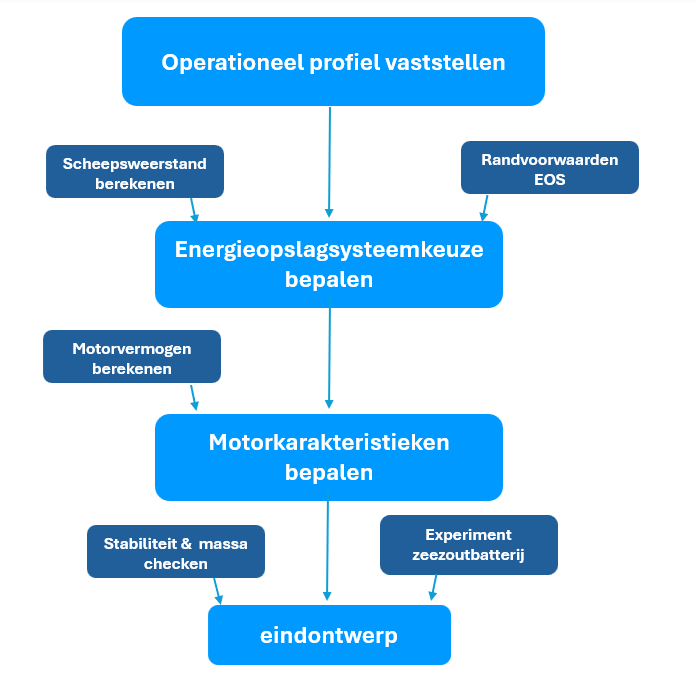
\includegraphics[width=0.8\linewidth]{chart V1.png}
    \caption{Stroomschema van dit project.}
    \label{fig:zijkant}
\end{figure}
